%Zarantonello Umberto 2021-04-30

\section{Applicazioni di Fisica Nucleare}

Fino agli inizi del secolo scorso si pensava che gli ambiti della fisica fossero piuttosto divisi e che, pur avendo un fondo comune, si potessero spiegare bene anche in modo indipendente.
Nel corso del 1900 con la rivoluzione della fisica questo sentimento di divisione iniziò a venire meno e si capì che gli ambiti potevano essere spiegati con un unica teoria di fondo.
Le ricerche attuali dimostrano che anche in ambito sperimentale le ricerche sono sempre più comuni, basti pensare a come la fisica nucleare, l'astrofisica e la cosmologia siano oggi comunicanti, a partire dalla ricerca dei neutrini per finire ai processi di fusione nucleare.
In questa sezione sono quindi raccolti alcuni argomenti del corso che non fanno rifermento propriamente alla fisica nucleare ma che ne prendono le basi per applicazioni in altri campi.

\subsection{Fisica Medica: Risonanza Magnetica Nucleare}
La risonanza magnetica è una tecnica di imaging medico non invasiva.
Si basa sul fatto che ad ogni protone è associato un piccolo campo magnetico associato al dipolo. 
Ponendo questi dipoli sotto l'azione di un campo magnetico forte, si avrà l'allineamento con il campo, sia nella stessa direzione che i direzione opposta.
\begin{equation}
E=-\bar \mu\cdot \bar B
\end{equation}
Ciò che si otterrà è che l'energia sarà minore se il campo e il dipolo sono solidali ($\mu\uparrow\  B\uparrow$), mentre sarà maggiore nel caso contrario ($\mu\uparrow\  B\downarrow$).
\begin{figure}

\end{figure}
La differenza di energia è pari a $\Delta E=\mu B$.
La risonanza in campo magnetico sfrutta esclusivamente nucleoni ma in altri ambiti possono essere usati anche gli elettroni e dalla formula sopra si può vedere come sia diversa nei due casi.

I valori del magnetone di Bohr e del magnetone nucleare sono 
\begin{equation}
\begin{split}
\mu_B=\frac{e\hbar}{2m_e}=9,3\times10^{-24}\frac{j}{T}=5,8\times10^{-5}\frac{eV}{T}\\
\mu_N=\frac{e\hbar}{2m_p}=5,0\times10^{-27}\frac{j}{T}=3,8\times10^{-8}\frac{eV}{T}
\end{split}
\end{equation}

La risonanza magnetica funziona che una volta applicato un campo magnetico i livelli energetici con spin up e down si dividono e fornendo una radiofrequenza con energia pari alla differenza di energia generata il mio campione assorbirà energia, e io sono sensibile all'energia assorbita. 

Dato un elettrone se applico un campo B=0,335T, ottengo che la differenza di energia sarà pari a $\Delta E=6,22\times 10^{-24}j$.
In questo caso la frequenza coinvolta (assorbita dall'elettrone) è pari a $\nu =9,4GHz$, ovvero nel campo delle microonde.

Nel caso del protone, ovvero quello usato in campo medico, c'è la necessità di applicare un campo magnetico molto più alto per portare ad una separazione sufficientemente visibile. 
Applicando un campo $B=2T$ ottengo $\Delta E=5,64\times10^{-26}j$, vi è quindi la necessità di una radiofrequenza dell'ordine di $\nu =\frac{\Delta E}{h}=85MHz$.

Quello che succede è che pongo il paziente in questi campi magnetici e faccio passare una radiofrequenza. 
L'assorbimento di questa radiofrequenza avviene in funzione della densità del materiale biologico.
Una cosa di cui devo tener conto è l'agitazione termica dei protoni, posso immaginare che maggiore è l'agitazione termica minore sarà il contrasto dell'immagine, una soluzione sarebbe abbassare la temperatura ma non potendo congelare il paziente non resta che sfruttare campi magnetici molto forti($\Delta E/KT$).
Il segnale che io rivelo è proporzionale alla densità di protoni, le zone più chiare sono quelle a più elevata densità di protoni.
Per avere una risoluzione spaziale, ovvero una tridimensionalità, applico un gradiente di campo magnetico minimo che produrrà una risonanza diversa a diverse frequenze di radiofrequenza generando una variazione ulteriore che mi permette di ampliare l'imaging.
Per andare ad aumentare il contrasto andrò a vedere la risposta temporale del campione.
Quando irradio il tessuto i protoni assorbendo energia passeranno da uno stato all'altro (spin-flip), se poi io fermo la radiazione e lascio il tessuto tornare allo stato fondamentale potrò poi misurare il tempo impiegato per la diseccitazione e avrò quindi informazioni addizionali sul tessuto che circonda il materiale in analisi.

\subsection{Cosmologia: Storia dell'universo primordiale}

La formazione degli elementi inizia da quello che chiamiamo Big Bang, che si tratta di questo evento singolare che ha dato origine all'universo visibile.
La nostra capacità di descrivere questo evento parte da un tempo di $10^{-43}s$, che si chiama tempo di Plank e corrisponde al momento in cui la forza di gravità si è separata da tutte le altre forze.
Questo tempo può in realtà essere espresso in tante forme, per esempio sotto forma di energia è pari a $10^{19}GeV$.
Diciamo che la forza di gravità si è separata dalle altre forze, poiché si è notato che, facendo un grafico con tutte la forze in funzione del tempo, tornando indietro nel tempo (ossia aumentando l'energia), tutte tendono ad avere la stessa intensità, si suppone quindi che all'istante iniziale tutte le forze fossero un'unica forza.
Prima dell'evento di separazione della gravità non si può spiegare quello che ci fosse.
Per andare oltre servirebbe una teoria quantistica della gravità.

La seconda forza che si è separata dalle altre è stata la forza nucleare forte.
In un periodo successivo che va da $10^{-36}s$ fino a $10^{-32}s$ si pensa ci sia stato un evento di espansione anomala (con una velocità più alta di quella della luce) chiamata inflazione.
Questa teoria serve a spiegare il fatto che la radiazione cosmica di fondo risulta termalizzata, ci sono infatti regioni dell'universo che hanno la stessa temperatura pur essendo impossibile che queste regioni abbiano comunicato tra loro, poiché non si sarebbero mai potute scambiare fotoni.
In questo tempo l'universo si è ingrandito di $30$ ordini di grandezza.

Le teorie che spiegano l'universo dal momento di separazione della forza di gravità fino al momento di inflazione sono dette teorie di grande unificazione (GUT) in quanto tutte le altre forze sono ancora unite.
Le teorie di maggiore sviluppo oltre il modello standard arrivano fino alla GUT.
Queste ci danno delle ipotesi su quello che potrebbe essere l'universo prima di questo periodo di grande unificazione.
Prima dell'inflazione deve esserci stato anche un meccanismo per cui la materia e l'antimateria si pongono in asimmetria.

Dopo il periodo inflazionistico ci deve essere stata la separazione tra forza debole ed elettromagnetica.
Il tempo a cui questo evento è avvenuto è pari a $10^{-12}s$ con un energia di $100GeV$.
Queste sono le energie massime raggiungibili attualmente dall'acceleratore più potente ossia l'LHCb del Cern ($10^{-13}s$).

A $10^{-6}s (200 MeV)$ si ha quello che viene chiamato $quark cofinement$ ossia questo è il momento in cui i quark da liberi si combinano portando alla creazione di materia e antimateria, fino a prima infatti ci si trovava in quello che è definito come il quinto stato della materia ovvero il plasma di quark e gluoni.
Questo periodo è anche quello di annichilazione materia antimateria che ha portato all'emissione della radiazione cosmica di fondo, inizialmente emessa come raggi gamma ma negli anni andatasi a raffreddare.
\'E quindi questo il momento in cui si viene a creare l'effettiva asimmetria tra materia e antimateria, dovuta ad una disparità di una particella ogni biliardo di particelle ma che comunque ha generato l'universo per come lo conosciamo.

Ad $1s$ dal Big Bang, con un'energia pari a $2MeV$ si ha il disaccoppiamento dei neutrini fossili.
Questi permeano l'universo come la radiazione cosmica di fondo ma sono estremamente difficili da rivelare in quanto come per la radiazione hanno perso energia con l'espansione dell'universo, arrivando ad una temperatura attuale di $2K$.
Riuscire a intercettare queste particelle sarebbe di grande aiuto per la comprensione dell'evoluzione dell'universo ma, essendo i neutrini particelle estremamente elusive anche ad alta energia, è difficile trovare un processo che riesca a coinvolgere dei neutrini a così bassa energia.

Il disaccoppiamento dei neutrini comporta anche il disequilibrio termico degli adroni, infatti questi sono la particella cardine del decadimento beta e quindi sono pure la particella che genera l'equilibrio termico tra protoni e neutroni.
Inizia quindi il decadimento dei neutroni.
In conseguenza si ha che a $3s$ inizia la nucleosintesi primordiale.
Il bilancio iniziale tra queste particelle non è equo a causa della disparità di peso tra le il protone e il neutrone, la distribuzione iniziale era di 
\[
0,76p+0,24n
\]
Questo processo dura dai $3$ ai $20$ minuti di storia dell'universo e interessa energie che partono da $200KeV$ per finire quando si raggiungono i $60KeV$.
Le particelle create sono il deuterio e l'elio
\[
p+n\to^2_1H\hspace{0.5cm}^2_1H+^2_1H\to^4_2He
\]
con una distribuzione di $75\%H$ e $25\%He$.
Come già visto non si vengono a creare nuclei più pesanti perché non esistono nuclei stabili con numero di massa $A=5$ e $A=8$.

Per avere un'evoluzione ulteriore bisogna andare a $380000$ anni dal Big Bang, quando la radiazione cosmica di fondo, generata ad $1s$ si disaccoppia dalla materia e viene emessa (conseguenza che gli atomi iniziano ad essere legati quindi non più in uno stato plasmatico).
La temperatura è di $4000K$ e l'energia di $0,5KeV$.

\subsection{Astrofisica: Nucleosintesi Stellare}

Gli elementi più pesanti dell'elio necessitano di processi più complessi di quelli della nucleosintesi primordiale perché devono superare i limiti posti dall'assenza di elementi stabili intermedi.
In generale c'è bisogno di energie più elevate per innescare processi di fusione che superino le barriere imposte dalla natura e queste energie sono ottenuta all'interno delle stelle grazie alle pressioni che si vengono a creare grazie alla forza di gravità.

Le stelle si dividono in tre categorie in base alla quantità di materiale metallico:
\begin{itemize}
\item stelle di terza popolazione: sono le prime stelle che si sono generate e presentano l'assenza di materiale metallico; proprio per il fatto di essere le stelle più antiche non sono ancora state osservate.
\item stelle di seconda popolazione: sono le stelle a basso contenuto metallico e identificate come la seconda popolazione generatasi.
\item stelle di prima popolazione: sono le stelle ad alto contenuto metallico; non bisogna lasciarsi trarre in inganno da "alto" in quanto la gran parte della stella rimane formata da idrogeno; ne fa parte anche il sole.
\end{itemize}

All'interno delle stelle non sono presenti neutroni quindi, a differenza della nucleosintesi primordiale, la reazione avviene per forza debole, il che rende la stella molto longeva rispetto a quello che sarebbe se le reazioni fossero più spontanee.

La reazione principale di funzionamento è illustrata nelle seguenti formule e parte dal decadimento protonico che presenta una sezione d'urto pari a $\sigma =10^{-47}cm^2$
\begin{equation}
\begin{split}
p&\longrightarrow n+e^++\nu_e\\
p+n&\longrightarrow ^2_1H\\
^2_1H+^1_1H&\longrightarrow ^3_2He+5,5MeV\\
^3_2He+^3_2He&\longrightarrow ^4_2He+2p+12,9MeV
\end{split}
\end{equation}

Un altro ciclo importante per il mantenimento della stella è il ciclo CNO, ottenibile solamente nelle stelle di prima popolazione perché possibile solo in presenza di un'alta metallicità.
\begin{equation}
\begin{split}
^{12}_{6}C+p &\longrightarrow ^{13}_7N\\
^{13}_7N &\longrightarrow ^{13}_{6}C+e^++\nu_e\\
^{13}_{6}C+p &\longrightarrow ^{14}_7N\\
^{14}_7N +p &\longrightarrow ^{15}_8O\\
^{15}_8O &\longrightarrow ^{15}_7N\\
^{15}_7N+p &\longrightarrow ^4_2He +^{12}_{6}C
\end{split}
\end{equation}
Come indica anche il nome quindi questo è un ciclo che porta alla creazione di elio tornando costantemente al carbonio iniziale.
Questo processo genera anche due neutrini che vengono osservati tra le emissioni solari e grazie ai quali si è teorizzata per la prima volta l'oscillazione dei neutrini.

\paragraph{Creazione di elementi più pesanti dell'$He$}

Come si può vedere dal grafico a causa dell'instabilità di certi elementi la distribuzione è particolare ed è interessante notare come gli elementi con la più alta quantità siano tutti a numero di massa pari.
\begin{figure}[h]
\centering
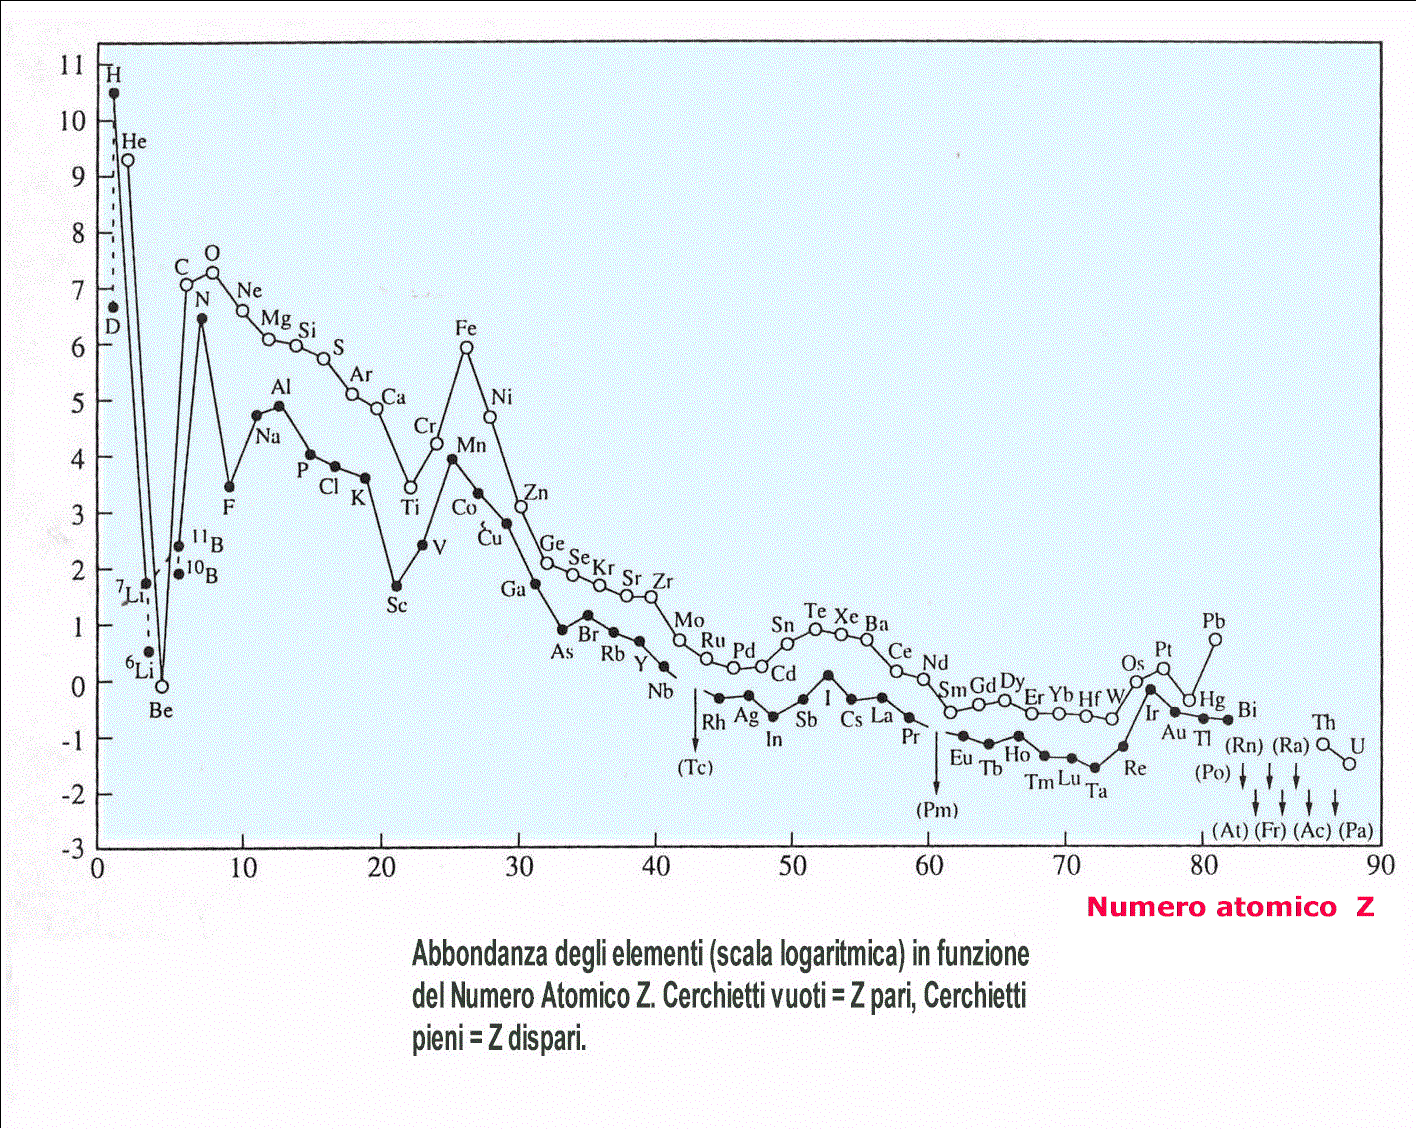
\includegraphics[width=180pt]{fig10_01}
\caption{Distribuzione degli elementi nell'universo}
\end{figure}

Finora non abbiamo spiegato il processo che ha portato alla creazione di elementi più pesanti dell'elio, ma è proprio per questo processo che si ritrova una distribuzione di elementi del tipo mostrato in figura.
Quando le stelle si avviano alla conclusione del ciclo vitale, gran parte dell'idrogeno è stato processato, quindi la stella non ha più energia sufficiente per contrastare la forza di gravità.
Per questo motivo la stella tende a collassare portando all'aumento della pressione interna.
Questo processo innesca la fusione degli atomi di elio con la formazione di Berilio.
\begin{equation}
^4_2He+^4_2He\longrightarrow ^8_4Be
\end{equation}
Che come detto più volte è instabile e decade in un tempo pari a $10^{-16}s$; inoltre la reazione di creazione del Berilio è endotermica quindi sfavorita.

C'è però un eccezione, se nel tempo di decadimento del Berilio questo entra in fase con un atomo di elio si può avere un ulteriore reazione di fusione che porta in uno stato eccitato del carbonio.
\begin{equation}
^8_4Be+^4_2He\longrightarrow ^{12}_6C^*
\end{equation}
che nella maggior parte dei casi ($99,6\%$) decade in tre atomi di elio
\begin{equation}
^{12}_6C^*\longrightarrow 3 ^4_2He
\end{equation}
Nei casi restanti, corrispondenti a $4$ ogni $10000$, si può avere quella che viene chiamata \emph{risonanza di Hayle}, dove il nucleo di carbonio di stabilizza tramite emissione gamma, e questo processo è proprio quello che porta alla creazione della materia più pesante dell'elio.

Tutti gli elementi più pesanti del carbonio poi vengono generati tramite l'assunzione progressiva di nuclei di elio (raggi alfa) ed ecco spiegata quindi la distribuzione concentrata maggiormente su nuclidi pari.
L'aggiunta di raggi alfa procede fino al nichel $^{56}_{28}Ni$ che essendo però proton rich decade spontaneamente
\begin{equation}
^{56}_{28}Ni\longrightarrow ^{56}_{27}Co\longrightarrow ^{56}_{26}Fe
\end{equation}
che è l'elemento con l'energia di legame più alta, dopo il quale serviranno altri processi endotermici per la creazione di elementi ulteriori.

La struttura stellare è quindi composta di una serie di sfere concentriche, ognuna con una concentrazione maggiore di un determinato elemento in base al peso di tale elemento.
Il nucleo stellare è solitamente composto in gran parte di ferro.

Bisogna considerare comunque che il sole è una stella medio piccola e quindi non riuscirà ad innescare questi processi ma si spegnerà semplicemente son la combustione totale dell'idrogeno.
Per innescare questi processi di collasso bisogna avere stelle ben più massive.

\paragraph{Processi di fusione oltre il ferro}

Per la creazione di materiali oltre il ferro la reazione è una combinazione di cattura neutronica e decadimento beta.
Si ha quindi che un nucleo assorbe dei neutroni che poi decadono in protoni generando nuovi nuclidi stabili.
La cattura neutronica può essere di due tipi: slow (rispetto al decadimento beta) o fast ( sempre confrontandola con il decadimento successivo).
Esiste una branca dell'astrofisica che studia esclusivamente questi processi nucleari chiamata astrofisica nucleare.
I processi di cattura slow possono essere  riprodotti in laboratorio per essere studiati mentre i processi fast hanno energie impossibili e avvengono solamente in esplosioni di supernove.

Facciamo ora un esempio di processo di emissione di neutroni.
\begin{equation}
^{13}_6C+^4_2He\longrightarrow ^{16}_8O+n
\end{equation}
Questi neutroni sono poi utilizzati in vari processi di cattura.
Un esempio di catena di tipo \emph{slow} è
\begin{equation}
^{56}_{26}Fe\to ^{57}Fe\to ^{58}Fe\to ^{59}Fe
\end{equation}
A questo punto però il processo si ferma perché l'ultimo isotopo è instabile e decade prima di poter catturare nuovamente, si ha quindi 
\begin{equation}
^{59}_{26}Fe\to ^{59}_{27}Co
\end{equation}
Per poi ripartire dal nuovo elemento con la cattura portando ad un nuovo decadimento beta e nuovamente ripartendo con la cattura.
\begin{equation}
^{60}Co\to ^{60}_{28}Ni\to ^{61}Ni\to ^{62}Ni\to \dots
\end{equation}
Il problema di questo processo, oltre alla lentezza con cui avviene, è il fatto che non riesce a spiegare tutti gli elementi esistenti in quanto è limitato agli elementi più vicini alla valle di stabilità.

L'unico modo di ottenere una produzione di neutroni massiccia, è all'interno di stelle estremamente massive.
Alla fine della vita di queste stelle, come già visto, avviene un collasso, seguito da un rinculo che va a ridistribuire la materia nello spazio.
Durante questo collasso che coinvolge energie altissime si ha un processo chiamato neutronizzazione che avviene tramite la fuzione di un protone e un elettrone 
\begin{equation}
p+e^-\longrightarrow n+\nu_e
\end{equation}
con quindi l'emissione di neutroni e neutrini.
Qui possono avvenire grandi eventi di cattura neutronica in grado di spiegare tutti i materiali esistenti in natura.

\subsection{Oltre il modello standard}
Quando la forza elettromagnetica e la forza gravitazionale sono confrontabili?

Prendiamo in considerazione due elettroni che si avvicinano e cerchiamo la distanza a cui le due forze sono confrontabili.
\begin{equation}
F_{em}=\frac{1}{4\pi\varepsilon_0}\frac{q_1q_2}{r^2}=K\frac{q_1q_2}{r^2}
\end{equation}
\begin{equation}
F_g=G\frac{m_1m_2}{r^2}
\end{equation}
Nel caso di due elettroni si avrà che $q_1=q_2=e$ e $m_1=m_2=m$.

Ragioniamo quindi sulla forza gravitazionale; introduciamo la lunghezza d'onda di Compton
\begin{equation}
p=\frac{h}{\lambda}\sim \frac{h}{r}
\end{equation}
L'energia dell'elettrone sarà quindi uguale
\begin{equation}
E=pc=\frac{hc}{r}
\end{equation}
Ma che può essere interpretata anche come
\begin{equation}
E=mc^2\to m=\frac{E}{c^2}=\frac{h}{rc}
\end{equation}
A questo punto si può esprimere la forza gravitazionale come 
\begin{equation}
F_g=G\frac{m^2}{r^2}=\frac{G}{r^2}\frac{h^2}{r^2c^2}=\frac{Gh^2}{r^4c^2}
\end{equation}

La forza elettromagnetica e la forza gravitazionale si eguaglieranno quando
\begin{equation}
K\frac{e^2}{r^2}=\frac{Gh^2}{r^4c^2}\longrightarrow r^2=\frac{Gh^2}{Ke^2c^2}
\end{equation}
Essendo questo raggio espresso solo in funzione di costanti fondamentali è possibile ricavarlo.
Un calcolo approssimativo restituisce
\begin{equation}
r=10^{-33}m
\end{equation}
Questo raggio, che si ottiene quando le due forze si eguagliano, corrisponde ad un'energia 
\begin{equation}
E=\frac{hc}{r}=10^7J=10^{17}GeV
\end{equation}
Per fare un confronto LHC raggiunge energie massime di $10^4GeV$.

Questa è un'energia che corrisponde al momento in cui tutte le forze erano unite e quindi un momento in cui i concetti di base della fisica erano completamente diversi.
Si suppone però che a quei tempi siano avvenuti fenomeni estremamente interessanti per l'evoluzione dell'universo e poter raggiungere tali energie potrebbe essere interessante.




